\subsubsection{Challenges in medical image processing for deep learning}
\label{sec:challenges}


In practice, multiple challenges must be addressed when developing deep learning algorithms for medical images:
1) handling metadata related to physical position and size,
2) lack of large labeled datasets,
3) high computational costs due to data multidimensionality and
4) lack of consensus for best normalization practices.
These challenges are very common in medical imaging and require certain features that may not be implemented in more general-purpose image processing frameworks such as Albumentations~\cite{buslaev_albumentations_2020} or TorchVision~\cite{paszke_pytorch_2019}.


\paragraph{Metadata}
\label{sec:metadata}

In computer vision, picture elements, or \textit{pixels}, which are assumed to be square, have a spatial relationship that comprises proximity and depth according to both the arrangement of objects in the scene and camera placement.
In comparison, medical images are reconstructed such that the location of volume elements, or cuboid-shaped \textit{voxels}, encodes a meaningful 3D spatial relationship.
In simple terms, for 2D natural images, pixel vicinity does not necessarily indicate spatial correspondence, while for medical images spatial correspondence between nearby voxels can often be assumed.

Metadata, which encodes the physical size, spacing, and orientation of voxels, determines spatial relationships between voxels~\cite{larobina_medical_2014}.
This information can provide meaningful context when performing medical image processing, and is often implicitly or explicitly used in medical imaging software.
Furthermore, metadata is often used to determine correspondence between images as well as voxels within an image.
For example, registration algorithms for medical images typically work with physical coordinates rather than voxel indices.

\cref{fig:metadata} shows the superposition of an \ac{MRI} and a corresponding brain parcellation~\cite{cardoso_geodesic_2015} with the same size ($181 \times 181$) but different origin, spacing and orientation.
A naïve user would assume that, given that the superimposition looks correct and both images have the same size, they are ready for training.
However, the visualization is correct only because 3D Slicer~\cite{fedorov_3d_2012}, the software used for visualization, is aware of the spatial metadata of the images.
As \acp{CNN} generally do not take spatial metadata into account, training using these images without preprocessing would lead to poor results.


\begin{figure}
  \centering

  \begin{subfigure}{0.24\textwidth}
    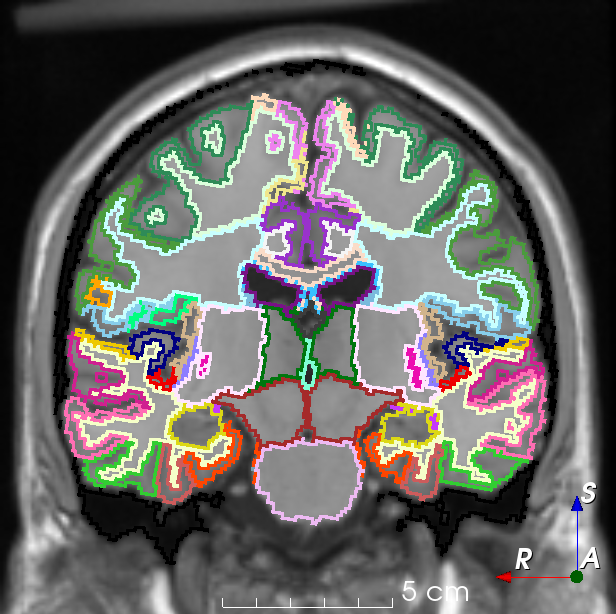
\includegraphics[width=\linewidth]{metadata_ok}
    \caption{}
    \label{fig:meta_ok}
  \end{subfigure}
  \hfill
  \begin{subfigure}{0.24\textwidth}
    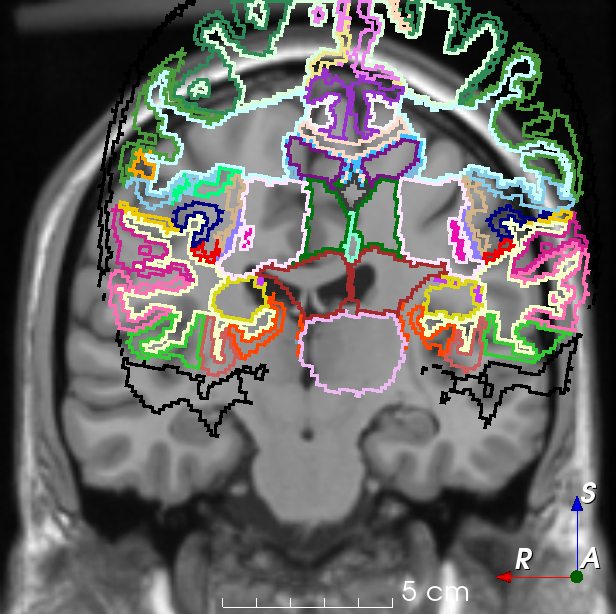
\includegraphics[width=\linewidth]{metadata_origin}
    \caption{}
    \label{fig:meta_origin}
  \end{subfigure}
  \hfill
  \begin{subfigure}{0.24\textwidth}
    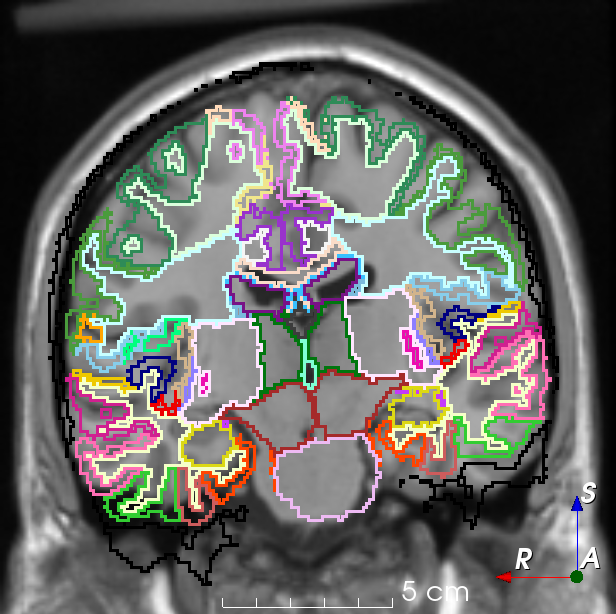
\includegraphics[width=\linewidth]{metadata_orientation}
    \caption{}
    \label{fig:meta_orientation}
  \end{subfigure}
  \hfill
  \begin{subfigure}{0.24\textwidth}
    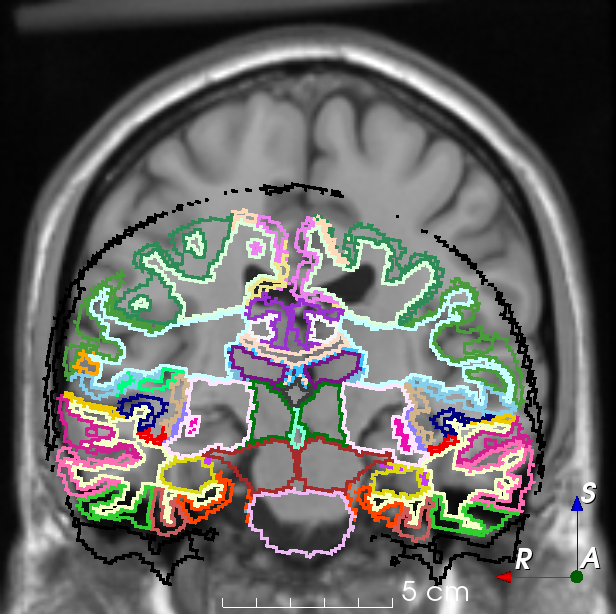
\includegraphics[width=\linewidth]{metadata_spacing}
    \caption{}
    \label{fig:meta_spacing}
  \end{subfigure}

  \caption[Importance of spatial metadata in medical imaging processing]{
    Demonstration of the importance of spatial metadata in medical image processing.
    The size of both the \ac{MRI} and the segmentation is $181 \times 181$.
    When spatial metadata is taken into account (\subref{fig:meta_ok}), images are correctly superimposed (only the borders of each region are shown for clarity purposes).
    Images are incorrectly superimposed if (\subref{fig:meta_origin}) origin, (\subref{fig:meta_orientation}) orientation or (\subref{fig:meta_spacing}) spacing are ignored.
  }
  \label{fig:metadata}
\end{figure}



Medical images are typically stored in specialized formats such as \ac{DICOM} or \ac{NIfTI}~\cite{larobina_medical_2014}, and commonly read and processed by medical imaging frameworks
such as SimpleITK~\cite{lowekamp_design_2013} or NiBabel~\cite{brett_nipynibabel_2020}.


\paragraph{Limited training data}

Deep learning methods typically require large amounts of annotated data, which are often scarce in clinical scenarios due to concerns over patient privacy, the financial and time burden associated with collecting data as part of a clinical trial, and the need for annotations from highly-trained and experienced raters.
Data augmentation techniques can be used to increase the size of the training dataset artificially by applying different transformations to each training instance while preserving the relationship to annotations.

Data augmentation performed in computer vision typically aims to simulate variations in camera properties, \ac{FOV}, or perspective.
Traditional data augmentation operations applied in computer vision include geometrical transforms such as random rotation or zoom, color-space transforms such as random channel swapping or kernel filtering such as random Gaussian blurring.
Data augmentation is usually performed on the fly, i.e., every time an image is loaded from disk during training.

Several computer vision libraries supporting data augmentation have appeared recently, such as Albumentations~\cite{buslaev_albumentations_2020}, or \texttt{imgaug}~\cite{jung_imgaug_2020}.
PyTorch also includes some computer vision transforms, mostly implemented as Pillow wrappers~\cite{wiredfool_pillow_2016}.
However, none of these libraries support reading or transformations for 3D images.
Furthermore, medical images are almost always greyscale, therefore colour-space transforms are not applicable.
Additionally, cropping and scaling are more challenging to apply to medical images without affecting the spatial relationships of the data.
Metadata should usually be considered when applying these transformations to medical images.

In medical imaging, the purpose of data augmentation is designed to simulate anatomical variations and scanner artifacts.
Anatomical variation and sample position can be simulated using spatial transforms such as elastic deformation, lateral flipping, or affine transformations.
Some artifacts are unique to specific medical image modalities.
For example, ghosting artifacts will be present in \ac{MRI} if the patient moves during acquisition, and metallic implants often produce streak artifacts in \ac{CT}.
Simulation of these artifacts can be useful when performing augmentation on medical images.


\paragraph{Computational costs}
\label{sec:computation}
The number of pixels in 2D images used in deep learning is rarely larger than one million.
For example, the input size of several popular image classification models is $224 \times 224 \times 3 = \num{150528}$ pixels (\SI{588}{\kibi\byte} if 32 bits per pixel are used).
In contrast, 3D medical images often contain hundreds of millions of voxels, and downsampling might not be acceptable when small details should be preserved.
For example, the size of a high-resolution lung \ac{CT}-scan used for quantifying chronic obstructive pulmonary disease damage in a research setting, with spacing $0.66 \times 0.66 \times 0.30$ mm, is $512 \times 512 \times 1069 = \num{280231936}$ voxels (\SI{1.04}{\gibi\byte} if 32 bits per voxel are used).


In computer vision applications, images used for training are grouped in batches whose size is often in the order of hundreds~\cite{krizhevsky_imagenet_2012} or even thousands~\cite{chen_simple_2020} of training instances, depending on the available \ac{GPU} memory.
In medical image applications, batches rarely contain more than one~\cite{cicek_3d_2016} or two~\cite{milletari_v-net_2016} training instances due to their larger memory footprint compared to natural images.
This reduces the utility of techniques such as batch normalization, which rely on batches being large enough to estimate dataset variance appropriately~\cite{ioffe_batch_2015}.
Moreover, large image size and small batches result in longer training time, hindering the experimental cycle that is necessary for hyperparameter optimization.
In cases where \ac{GPU} memory is limited and the network architecture is large, it is possible that not even the entirety of a single volume can be processed during a training iteration.
To overcome this challenge, it is common in medical imaging to train using subsets of the image, or image \textit{patches}, randomly extracted from the volumes.

Networks can be trained with 2D slices extracted from 3D volumes, aggregating the inference results to generate a 3D volume~\cite{lucena_convolutional_2019}.
This can be seen as a specific case of patch-based training, where the size of the patches along a dimension is one.
Other methods extract volumetric patches for training, that are often cubes, if the voxel spacing is isotropic~\cite{li_compactness_2017}, or cuboids adapted to the anisotropic spacing of the training images~\cite{nikolov_deep_2018}.


\paragraph{Transfer learning and normalization}

One can pre-train a network on a large dataset of natural images such as ImageNet~\cite{deng_imagenet_2009}, which contains more than 14 million labeled images, and fine-tune on a custom, much smaller target dataset.
This is a typical use of transfer learning in computer vision~\cite{weiss_survey_2016}.
The literature has reported mixed results using transfer learning to apply models pretrained on natural images to medical images~\cite{cheplygina_cats_2019,raghu_transfusion_2019}.

In computer vision, best practice is to normalize each training instance before training, using statistics computed from the whole training dataset~\cite{krizhevsky_imagenet_2012}.
Preprocessing of medical images is often performed on a per-image basis, and best practice is to take into account the bimodal nature of medical images (i.e., that an image has a background and a foreground).

Medical image voxel intensity values can be encoded with different data types and intensity ranges, and the meaning of a specific value can vary between different modalities, sequence acquisitions, or scanners.
Therefore, intensity normalization methods for medical images often involve more complex parameterization of intensities than those used for natural images~\cite{nyul_standardizing_1999}.
